В этой секции рассмотрим сравнение описанных выше подходов. \cite{poletto1999}
Будем сравнивать как различия во времени компиляции программы,
так и влияние на производительность во время исполнения.

\subsection{Время компиляции}

На рисунке~\ref{fig:compile_bench} представлен график времени компиляции.
На вертикальной оси отмечены затраты на компиляцию в циклах на сгенерированную инструкцию.
Чем больше значение тем больше затраты.
По горизонтальной оси отложены различные тесты.
Для каждого теста есть 3 столбца.
Первый столбец \textbf{U} --- алгоритм распределяющий регистры при помощи подсчета количества использований.
Второй столбец \textbf{L} --- линейной аллокации.
Третий столбец \textbf{C} --- раскраски графа.
Так как столбец \textbf{U} нас не интересует, то комментировать его не будем.
Горизонтальные столбцы разделены на 3 части:

\begin{enumerate}
	\item \textbf{Анализ живности}.

	\item \textbf{Подготовка к распределению регистров}: Для \textbf{L} это расчет интервалов жизни,
	для \textbf{C} построение графа зацепленности.
	
	\item \textbf{Распределение регистров}: Для \textbf{L} это проход по интервалам, для \textbf{C} это раскраска графа.
\end{enumerate}

\begin{figure}[h]
	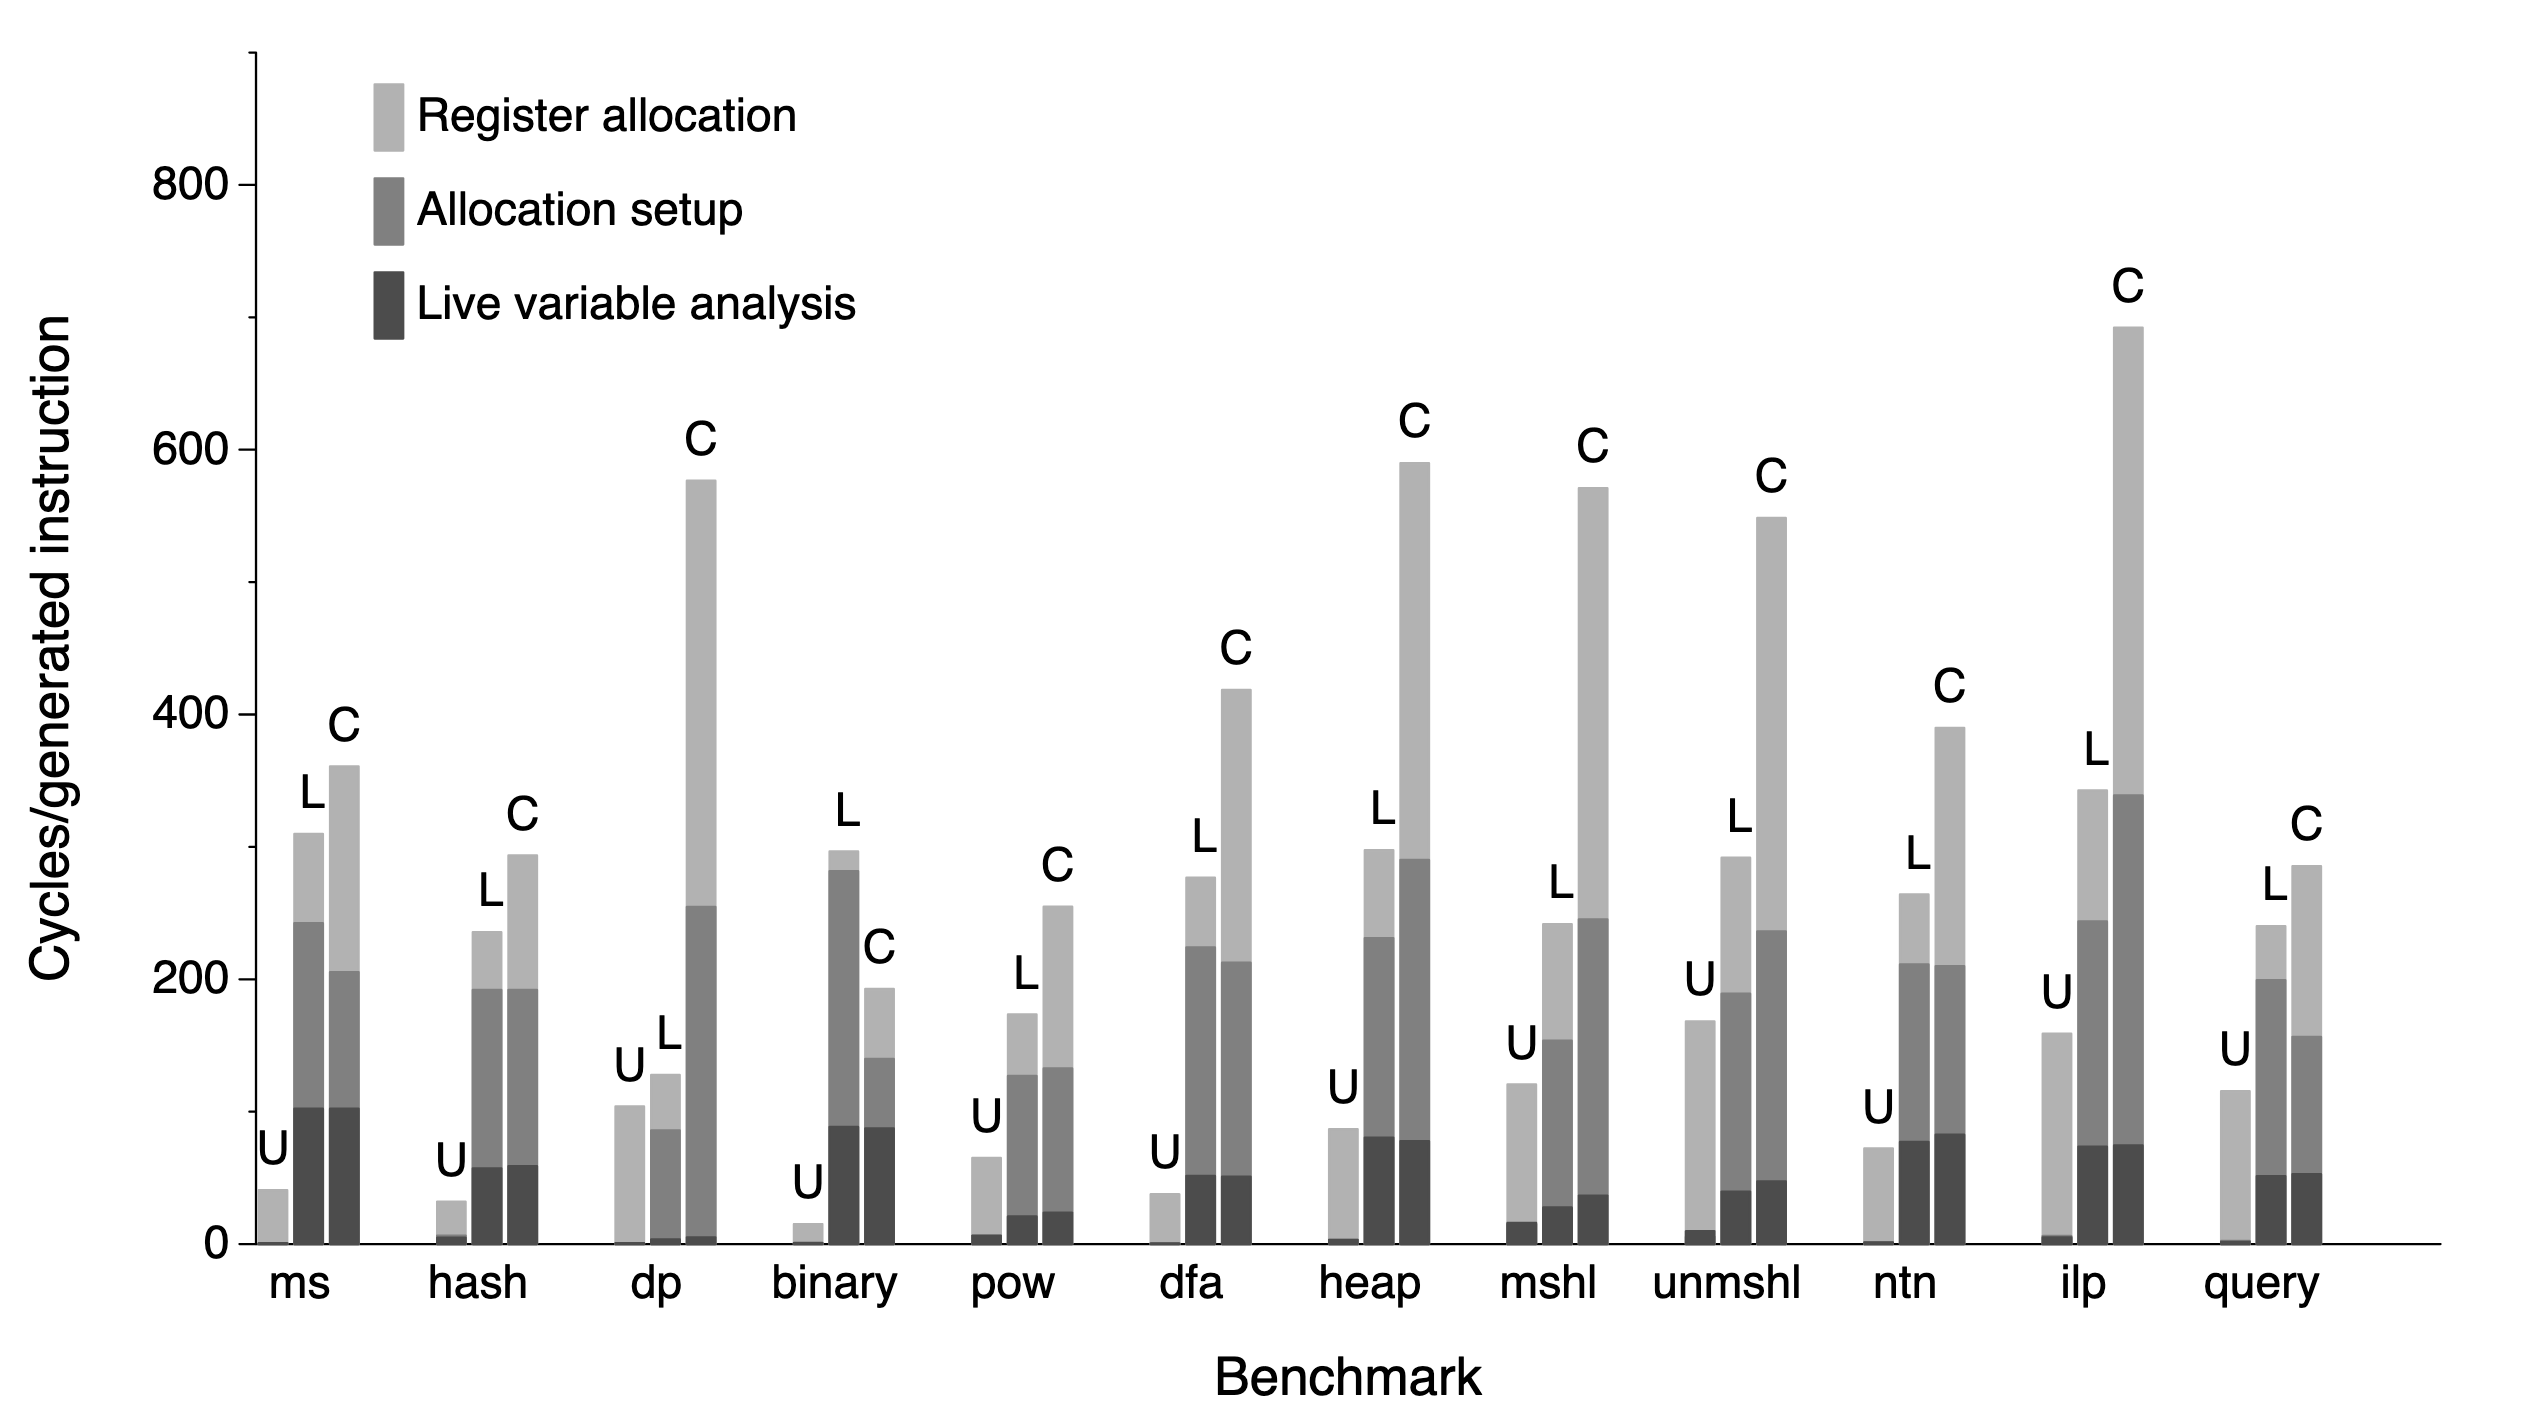
\includegraphics[width=\textwidth]{compile_time.png}
	\caption{Время компиляции}
	\label{fig:compile_bench}
\end{figure}

Видно, что практически для всех тестов алгоритм линейной аллокации быстрее чем алгоритм раскраски.
Интересные значения можно наблюдать в тесте binary.
Такие результаты объясняются тем, что в этом тесте небольшое количество переменных и очень много ветвлений.
В этом случае построить небольшой граф зацепленности быстрее, чем анализировать длинные интервалы жизни.
Однако стоит отметить, что время распределения регистров в этом тесте все же быстрее для линейной аллокации.

\subsection{Время исполнения}

На рисунке~\ref{fig:run_time} представлены результаты тестирования программ,
скомпилированных при помощи различных алгоритмов аллокации регистров.
В таблице представлены четыре алгоритма, нас интересуют только Linear scan и Graph coloring.
Значения в скобках представляют отношение времени исполнения метода,
скомпилированного с данным алгоритмом, к времени исполнения метода,
скомпилированного с алгоритмом раскраски графа.

Видно, что результаты линейной аллокации отличаются в пределах 10\%
от алгоритма раскраски графа.

\begin{figure}[h]
	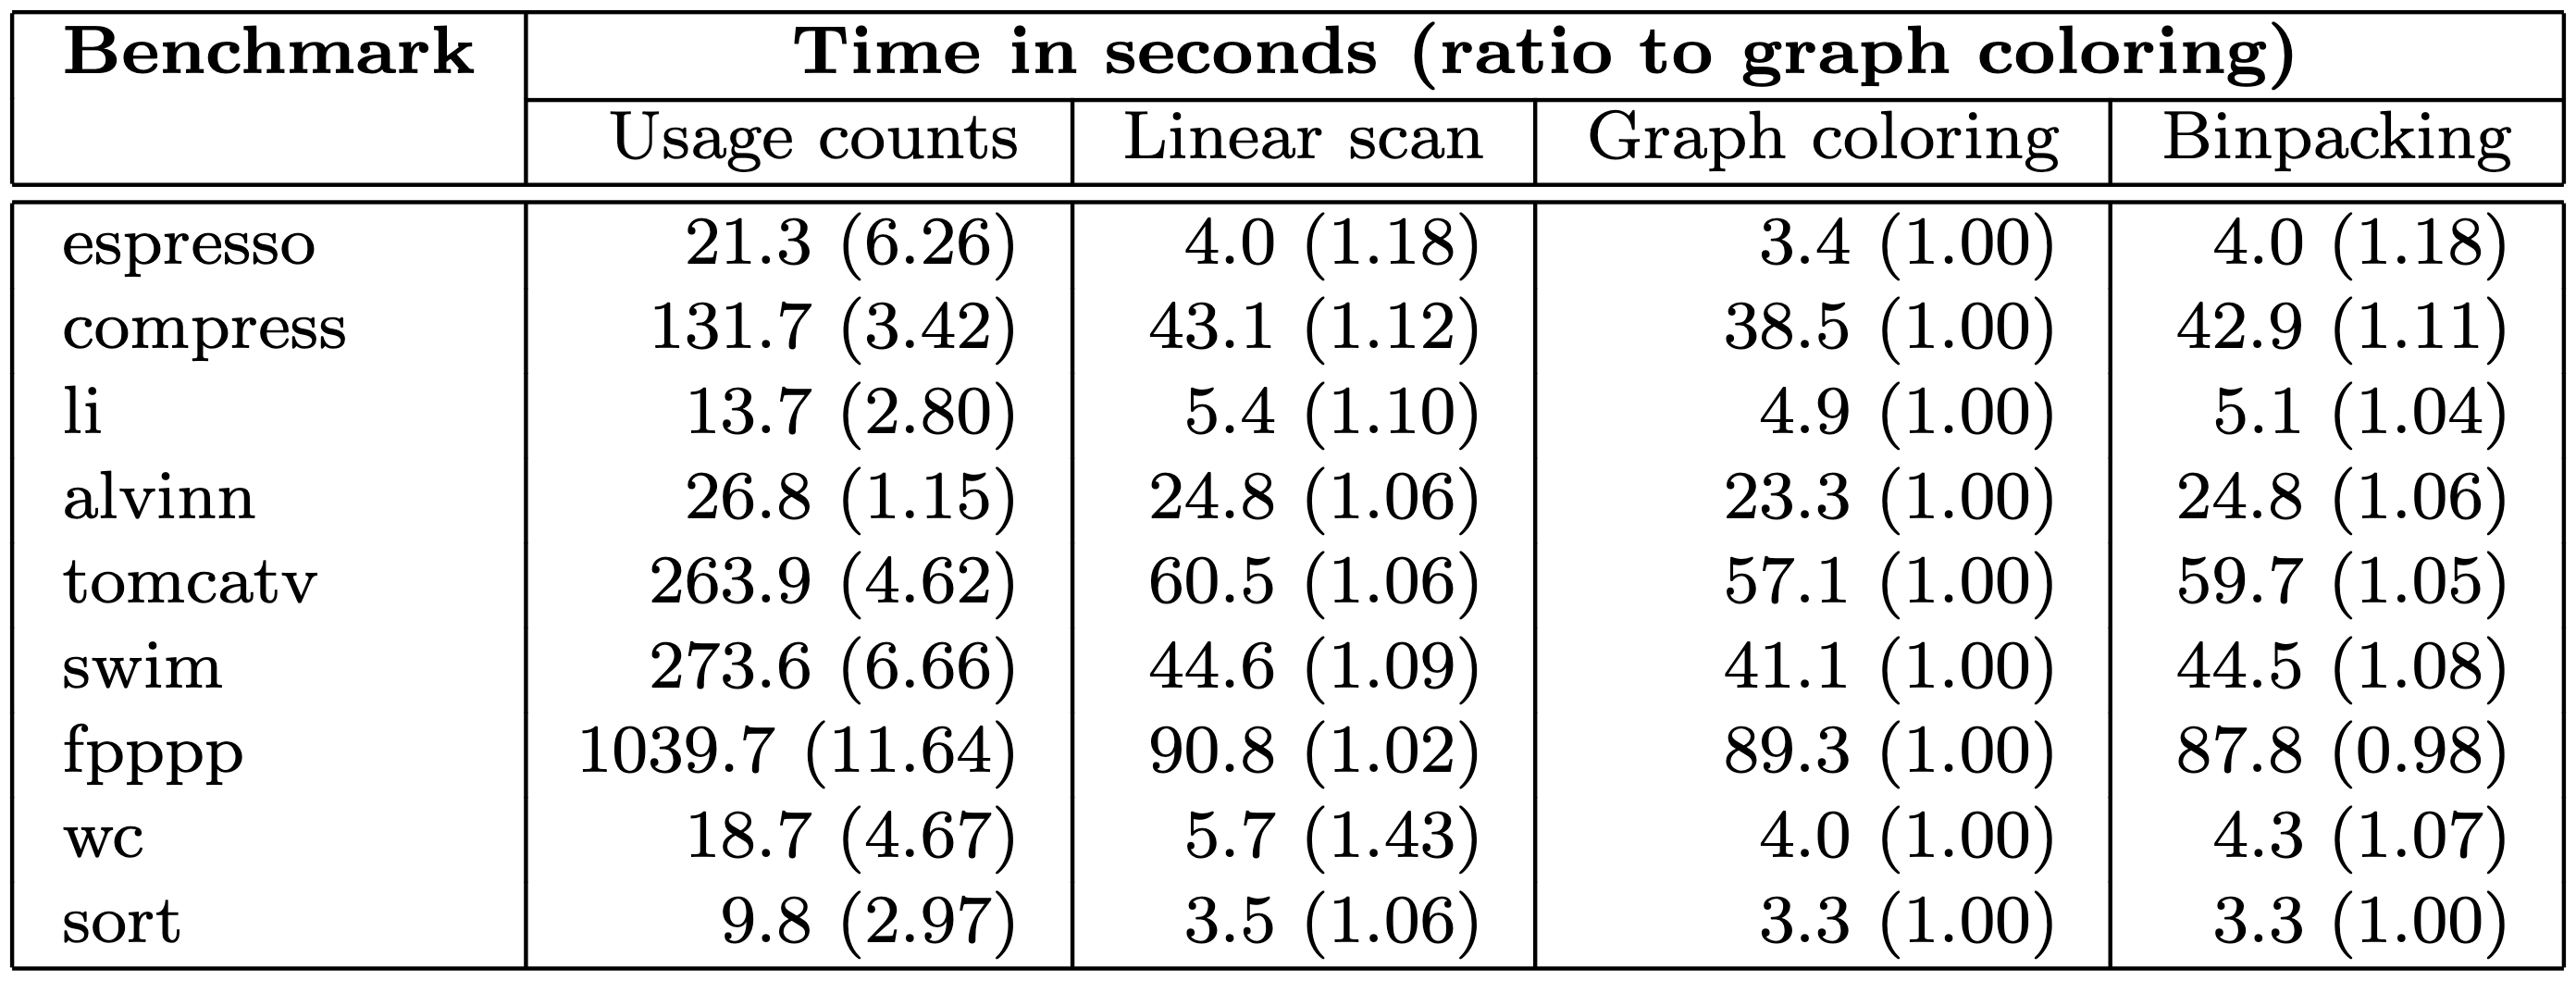
\includegraphics[width=\textwidth]{run_time.png}
	\caption{Время исполнения}
	\label{fig:run_time}
\end{figure}


